\chapter{Literature Review} \label{ch:review}
Low-resolution thermopile-array sensors (LR-TAS) have been widely used in health-caring and indoor monitoring because of the feature of preserving privacy. According to the final objective, the related literature could be roughly classified into three categories: indoor localization and gesture estimation \cite{multi,karayaneva2018use,jeong2014probabilistic},
room surveillance \cite{gonzalez2013using,thermosense,basu2015tracking,IRTAS16x4}
or human object tracking and event counting \cite{mika,firstflow,melexis,virtualtrack}.
Most of the literature proposed a two-layers algorithm structure, which consists of an object detection layer and an activity classification layer. Regardless of the different final goal of the researches, several similar ideas are found in the object detection algorithms, which has inspired our design. The later data processing procedure is more task-specific and only the literature in the last category is highly related to our design.

Before we dive into the related literature, it is worth mentioning that there are already several commercial products that could track and count humans \cite{irisys,flir}. But the work principles of these products are not revealed. Moreover, they cannot output an articulate number of human counts and are often applied in mass population monitor for example in supermarkets.

\section{Detection Algorithms}
In the active pixel detection phase, the algorithm needs to distinguish a human from the background, namely to answer the question of ``Which pixels are occupied by a human?''

\citeauthor{mashiyama2015activity} \cite{mashiyama2015activity} rearrange the pixels by their reading values in descending order, and take a heuristic that the first $n$ pixels could be human, having a prior knowledge that a human usually takes up $n$ pixels in a scene. They also compare the average temperature of the first $n$ pixels with the rest pixels, only when the difference is large enough the first $n$ pixels are considered a human. This method has several drawbacks. The most obvious issue is that it can only detect one person. Moreover, the algorithm depends heavily on the prior knowledge threshold $n$, so it lacks the flexibility to detect different people with different figures. Finally, \citeauthor{trofimova2017indoor} \cite{trofimova2017indoor} has re-conducted the research and pointed out that it is very hard to determine the threshold.

\citeauthor{trofimova2017indoor} \cite{trofimova2017indoor} has also proposed their detection algorithm, which makes use of the on-board thermistor to estimate the environment temperature. They found that there is an approximately linear relation between the IR array temperature and the thermistor temperature, which indicates that any higher reading that breaks this linear relation is probably caused by a human. Since the sensor they use has a reading deviation up to $\pm 2.5^{\circ}C$, a larger deviation from the thermistor temperature is considered a activated pixel. This method is able to detect activated pixels individually. But from temperature readings alone, an IR-TAS cannot distinguish humans from other heat emitters such as computers or heaters.

Another way to separate a human from the background is to fully exploit the whole image frame. If a human is the only heat source in a thermal image, it is almost safe to assume that the body temperature is higher than the ambient temperature. Therefore, the human body and the background are naturally separated by temperature. Otsu's method could be applied to each frame individually to find out a threshold, such that pixels with a higher temperature are considered occupied by a human \cite{firstflow}.

Otsu's method provides good segmentation result but its low speed may be a drawback when real-time performance is required. The average temperature and standard deviation of a thermal image could also be used to calculate the threshold between fore- and backgrounds. \citeauthor{virtualtrack} \cite{virtualtrack} have proposed a simple algorithm based on the average temperature: any pixels with a temperature in the range of average temperature $\pm 3.0^\circ C$ are regarded as potential human objects and the rest pixels in the same frame are regarded as background.
%TODO: 解释一下virtual track作者如此选定阈值的原因
They further calculate the average temperature of fore- and background respectively, denoted as $T_o$ (object temperature) and $T_a$ (ambient). Next, a measurement temperature ($T_m$) is calculated by the following formula \autoref{eq:segmentbyavg}, where $S_o$ is the size of the object and $S_p$ is the total pixel number of one frame. A pixel that is $3^\circ C$ higher than $T_m$ is regarded as non-human heat source and will be excluded from object list.
\begin{equation}\label{eq:segmentbyavg}
  T_m = T_a + (T_o-T_a)*\frac{S_o}{S_p}
\end{equation}

Similarly, \citeauthor{jeong2014probabilistic} \cite{jeong2014probabilistic} purpose a global adaptive threshold using information of a single image frame. They exploit the fact that a too low standard deviation of an thermal image suggests it contains noises only. The purposed threshold is shown in \autoref{eq:segmentbystd}, where Max and Mean are the maximum and mean value in one frame, and SD is the standard deviation.
\begin{equation}\label{eq:segmentbystd}
  Threshold = (Max-Mean)*\left(0.025+\frac{0.85}{Max-Mean+1}\right) + Mean - 0.7\times SD
\end{equation}

Beside the aforementioned methods, a large group of detection algorithms fall into background substraction \cite{backgroundsubsurvey}, see \autoref{fig:backgroundsub}. This method maintains a background model in the processor's memory. A pixel is regarded active if its reading deviates from the stored background significantly. Instead of a global threshold, background substraction allows different regions of a camera FOV having different thresholds, which may be useful when there is a known heat source that should be ignored. Though the background substraction technique is more commonly used in RGB image data, transferring it to thermal image data also shows impressive results.
\begin{figure}
  \centering
  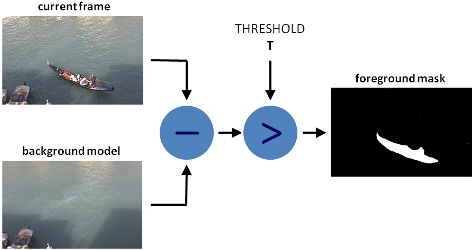
\includegraphics[width=0.8\textwidth]{figures/Background_Subtraction.png}
  \caption{A general idea of background substraction. Credit: \cite{opencvBackgroundSub}}\label{fig:backgroundsub}
\end{figure}

A simple implementation of background substraction is comparing the input image with a fix background. \citeauthor{basu2015tracking} \cite{basu2015tracking} collect more than 100 sample frames without humans, and use the average temperature as the background reference. \citeauthor{firstflow} \cite{firstflow} measure the background temperature only once when the device starts up, and take the assumption that the thermal background remains stable in a long term afterwards.

A fixed background may give acceptable result when the ambient temperature in the test environment does not vary. Under most circumstances, a background model that could adapt to the varying environment is desired. This could be done by a continuous update of the background pixels. After the fore- and background segmentation of each image frame, those pixels that do not exceed the background temperature will be merged into the background \cite{melexis,IRTAS16x4}, while those pixels that are considered as object do not contribute to the background model. The related formula is shown in \autoref{eq:backgroundupdate}:
\begin{equation} \label{eq:backgroundupdate}
\begin{split}
\mu_n[\mathbf{x}] & = \mathbf{1}\left(T_n[\mathbf{x}]\in B\right)\left[\alpha T_n[\mathbf{x}]+(1-\alpha)\mu_{n-1}[\mathbf{x}]\right]
  \\&+\mathbf{1}\left(T_n[\mathbf{x}]\in F\right) \mu_n[\mathbf{x}]
\end{split}
\end{equation}
where fore- and background are denoted as $F$ and $B$ respectively, $\mathbf{1}(\cdot)$ is the indicator function, and $\alpha \in (0,1)$ is the update rate.

The dynamic background learning method will dissolve an object that does not move for a long time into the background, which may be an advantage and drawback at the same time. When there is an unexpected non-human heat source in the camera view, the unanimated object could be ignored and do not influence detection judgements. On the other hand, a human will also be undesirably ignored if he stays still, which may brings about difficulties to the following algorithms. In order to detect humans only, \citeauthor{thermosense} \cite{thermosense} attached a PIR (passive infrared) sensor to their project in addition to the IR camera. PIR sensors are based on a principle of pyroelectric that is different from thermopile and can only detect heat movements. The authors assume that humans will not keep still for 15 minutes. The thermal camera will only capture and update the background if the PIR sensor does not sense a movement in such a period.

Finally, some researchers have explored machine learning (ML) methods for human object detection \cite{multi,karayaneva2018use}. But these methods will not be elaborated in this section because we want to concentrate on traditional CV methods.

\section{Tracking Algorithms}
After the human objects are detected and located, the task of a tracking algorithm is to assign a consistent label to the same object throughout the sequence of video images \cite{tang2010hybrid}. Following a bottom-up approach, four questions need to be answered to define an object tracker: what's the suitable (shape) representation of the object, what are the other features (color, texture, etc.) used to represent the object, how is the object detected, and how is it tracked \cite{trackingsurvey}. According to our discussion in the last section, the first and the third questions are already answered. To be more specific, we use pixel active/ inactive states to indicate whether a pixel is occupied by the human, which corresponds to the silhouette representation in \autoref{fig:objectrepresentation} (i). However, this blob representation could be simplified to other simpler representations such as a point representation after a feature extraction procedure, and is not necessarily the final input of the tracker.
\begin{figure}
  \centering
  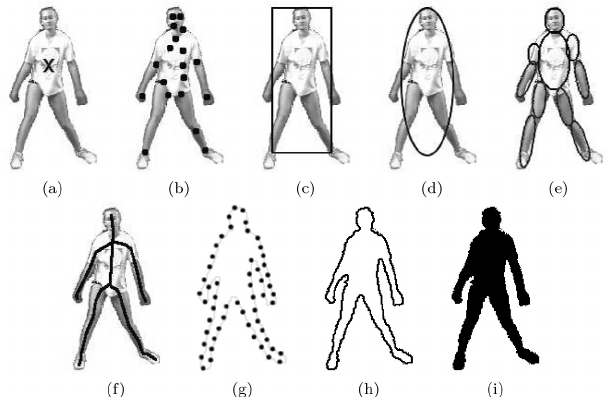
\includegraphics[width=0.8\textwidth]{figures/Object-representations.png}
  \caption{Different representations of objects. Credit: \cite{trackingsurvey}}\label{fig:objectrepresentation}
\end{figure}

\citeauthor{firstflow} \cite{firstflow} abstract the detected blob into a single point which has the largest distance to the background, and use this point as human body location. By tracking, the same label is assigned to a new blob if its distance to a previously seen blob is less than 10\% of frame width. In addition to the spatial constraint, the authors use a temperature feature to mark a blob, two blobs in sequential frames are considered the same person if their temperature difference is less than $1^\circ C$.

\citeauthor{mika} \cite{mika} also use the blob centroid to represent the human body location. Because the original resolution of the used IR camera is too coarse (only 8 by 8), they need to interpolate the image to $71\times71$ for tracking). Note that for a camera with $8\times8$ resolution, a spacial difference threshold of 10\% of the frame width is less than 1 pixel, which is impossible. Instead of matching the current position of a human body with a previously seen position directly, the authors smoothen the location updating with a Kalman filter \cite{kalmanfilter}. Similar tracking algorithms that are based on nearest neighbour association and Kalman filter can also be found in \cite{melexis,virtualtrack}.

By multiple blob association in one scene, a common challenge is to track merging/ splitting blobs correctly. When two people occur in the same frame, it is required that their blob representations have at least one pixel distance, otherwise the two blobs will be regarded as one large blob. Due to the low-resolution nature of IR-TAS, a gap of one pixel in the final image typically means some tens of centimeters between two people \cite{mika}. This issue is very hard to deal with in the tracking layer, which forbids tracking more than two people (because two people already amount to more than half of the camera view) or tracking any scenarios that two people may stand close, even for a short period of time.

An attempt to solve the issue is proposed by \cite{firstflow}. If one blob is large enough to be two merged blobs (larger than 30\% of frame's area), the background temperature threshold will be increased continuously at a step of $0.25^\circ C$ until a gap between two blobs emerges or the blob size shrinks to less than 10\% of frame area.

\citeauthor{virtualtrack} \cite{virtualtrack} try to solve the issue in the tracking layer. When two blobs merge, virtual trajectories will be created for both object with their previous positions and velocity. The merged human objects will be further propagated with their last seen velocity until the two blobs split. When the actual location points for both blobs are available again, the object position will be associated with an object label if it appears on the expected position given by a virtual trajectory. Since the positions in a virtual trajectory may deviate from the real ones significantly, the virtual trajectory will be replaced by a smoother back traced trajectory which connects the last actual position before merging and the first position after splitting. \autoref{fig:virtualpath} demonstrates the virtual trajectory tracking process.
\begin{figure}
  \centering
  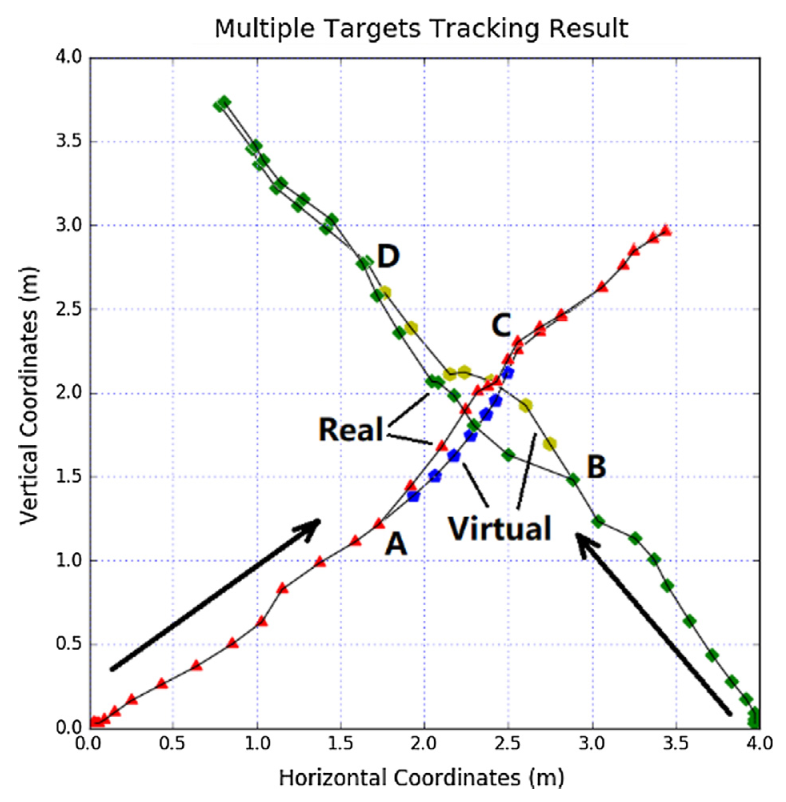
\includegraphics[width=0.5\textwidth]{figures/virtualpath.PNG}
  \caption{Multiple objects tracking result using virtual trajectory. Credit: \cite{virtualtrack}}\label{fig:virtualpath}
\end{figure}

Overall, we notice that a few related works have solved the aforementioned issue. We argue that two people moving in opposite direction through a doorway is a common scenario. Though people tend to keep a social distance of several tens of centimeters in a public space, at a narrow doorway they usually tilt the body to pass simultaneously rather than waiting the other to pass. Inevitably, the result of such a scenario will be a merged blob, which should be taken into consideration by the tracker's initial design.





